\section{Machine Learning Methods}\label{sec:machine-learning-methods}
Machine Learning Methods is a very broad term that over the last years, with the growing popularity of Neural Networks, got mixed with the more general term Artificial Intelligence.
The chapter will address the theory behind the "Modeling", "Training" and "Evaluation" steps in the Machine Learning Project Pipeline (\figref{fig:pipeline}).
Starting with a brief introduction on conventional ML methods such as \nameref{subsec:linear-regression} and \nameref{subsec:support-vector-machines}, then introducing algorithms that got very popular over the last few decades, such as \hyperref[subsec:neural-networks]{Artificial Neural Networks} and \nameref{subsec:cnn}.\\
After discussing the "Modeling" aspect an outlook on the "Training" and "Evaluation" of these models based on "\nameref{subsec:losses}" and "\nameref{subsec:metrics}" is given.
Then finishing with a short description on a method of finding right parameters for the selected models called "\nameref{subsubsec:hpo}".
The content of this chapter is a summary of the detailed explanations found in Aurélien Géron's "Hands-on Machine Learning with Scikit-Learn, Keras \& Tensor\-Flow"~\cite{handsOn}, combined with other books~\cite{ml-book}, lectures and paper resources.

\subsection{Tasks}\label{subsec:tasks}
Using ML a wide range of tasks can be tackled, starting from predicting house prices in a specific area to detecting cancer based on blood test values.\\
As stated in "\nameref{subsec:datasets}", the $N$ components of the feature vector $\mybold{x}^{(m)}$ used here for all tasks are pixel values from images.
All of these tasks can be described using a function $T$.\\
Let $T$ be the task function
$T: \R^{N} \rightarrow \R^K, \mybold{x^{(m)}} \mapsto \mybold{\hat{y}^{(m)}}$, with $K$ the number of output values of the prediction $\mybold{\hat{y}^{(m)}}$ for the $m$-th input $\mybold{x^{(m)}}$.
A pixel $\mybold{p}$ represents a color vector $\mybold{p}=(p_R, p_G, p_B)^T$, with $p_R, p_G, p_B \in \{0, 1,\ldots, 255\}$.
Images are two dimensional, they have a width $w$ and a height $h$ and most of the time their values differ between images.
For all ML methods the input values need to be scaled to the same dimensions, as stated in "\nameref{subsubsec:data-format}".

\subsubsection{Classification}
Classification is the task of predicting class labels $\mybold{\hat{y}^{(m)}}\in\R^K$ for a given input $\mybold{x^{(m)}}\in\R^N$.
The classification task can be subdivided into binary, multilabel
~\footnote{
    Multilabel classification is sometimes also called \textit{multinomial} classification.
}
and multioutput classification.
Binary classification focuses on detecting the probability of a given input belonging to a class or not and multioutput classification predicts probabilities, with a total probability of $100\%$, for a predefined set of classes.
Multilabel classification, on the other hand, predicts independent probabilities for multiple potential outputs, in contrast to multioutput the resulting probabilities do not necessarily sum up to $1.0$.
Here, multioutput classification is applied and described further.\\
As introduced, multioutput classification is the task of predicting a class out of $K$, here $K=5$, given classes for an given input $\mybold{x}^{(m)}$.
Let $T_c$ be the multioutput classification task function
\begin{align}
    T_c: \R^{N}\rightarrow [0,1]^{5}, \mybold{x^{(m)}} \mapsto \mybold{\hat{y}^{(m)}}
\end{align}
 with $\mybold{\hat{y}^{(m)}}_k$ the predicted probability of class $k$ for the $m$-th input $\mybold{x^{(m)}}$.

\subsubsection{Regression}
Regression, on the other hand, maps a given input onto one or many real numbers.
As in "\nameref{subsec:manual-labeling}" introduced, the regression task of predicting BB coordinates requires an output vector $\mybold{c^{(m)}} = \left(y_{\min}^{(m)}, x_{\min}^{(m)}, h^{(m)}, w^{(m)}\right)^T$, hence, a multi-output regression.\\
Therefore, let $T_r$ be the regression task function predicting values in shape \eqref{eq:bb}
\begin{align}
 T_r: \R^{N}\rightarrow \R^{4}, \mybold{x^{(m)}} \mapsto \mybold{c^{(m)}}\quad .
\end{align}


\subsection{Training Algorithms}\label{subsec:training-algorithms}
Commonly used across the Machine Learning scene are supervised algorithms for the problem of localization and classification of objects in image data. Apart from supervised learning algorithms there are also unsupervised, reinforcement and semi-supervised learning algorithms.
Supervised learning algorithms get trained on a stream of training samples, as in "\nameref{subsec:datasets}" introduced.
Here, the samples have the shapes \eqref{eq:regression-sample}, \eqref{eq:classification-sample} and \eqref{eq:1-stage-sample}.
During the training phase, the algorithm will compare the true values of each sample to the result of the prediction through the model for a given sample to its true value. This will be described in detail in "\nameref{subsec:losses}".\\
\textbf{Unsupervised learning} algorithms on the other hand do not get trained based on sample pairs $S^{(m)}$, they get trained on just the input values $\mybold{x^{(m)}}$.\\
Algorithms for \textbf{semi-supervised learning} rely on a mixture of labelled and unlabelled training data.
A common example would be a group of people that is recurrently visible in images.
In order to train the algorithm to detect specific people within different images, the annotator needs to provide a single labelled sample and the algorithm is capable of clustering the following images together in which those people appear.\\
\textbf{Reinforcement learning} algorithms on the other hand work completely differently to the (semi-/un-) supervised algorithms.
For this kind of algorithms, an agent explores a given environment and learns policies by gaining rewards or penalties for actions.
Along the way, the agent will eventually find the \textit{cheapest} or \textit{most rewarding} path of actions through the environment.\\
In the following, supervised learning algorithms will be discussed in detail, and a general overview given on how to train different kinds of supervised learning algorithms that are able to generalize the given task of localization and classification of insects in images.

\subsection{Linear Regression}\label{subsec:linear-regression}
Linear Regression (LinReg) is one of the standard supervised learning methods most often employed in classification and regression tasks, here LinReg will be applied to predict approximated Bounding Boxes $\mybold{\hat{y}^{(m)}}\in\R^4$ for an input $\mybold{x^{(m)}}\in\R^N$ and therefore solve a mutli output regression task.\\
LinReg finds a linear function that models the training set.
To perform a prediction of the $k$-th BB-coordinate of the $m$-th input – $\hat{y}^{(m)}_k$ – using a Linear Regression Model the weighted sum of the input values $\mybold{x^{(m)}}$ needs to be computed and added to a bias term $\omega_{0,k}$
\begin{align}
    \hat{y}^{(m)}_k = \omega_{0,k} + \omega_{1,k} \cdot x^{(m)}_1 + \ldots + \omega_{N,k} \cdot x^{(m)}_N
\end{align}
with $x^{(m)}_n$ the $n$-th component of $\mybold{x}^{(m)}\in \R^N$, $\omega_{0, k}$ the bias of the $k$-th output and $\omega_{n,k}$ for $n=1,\ldots, N$ the corresponding weights.
In vectorized form
\begin{align}
    \hat{y}_k^{(m)} =
    \skr{\mybold{\omega_k}, \mybold{x^{(m)}}} + \omega_{0, k}
\end{align}
with weights $\mybold{\omega_k}=\left(\omega_{1,k}, \omega_{2, k}, \ldots, \omega_{N, k}\right)^T$, $\mybold{x^{(m)}} = \left(x_1^{(m)}, x_2^{(m)}, \ldots, x_N^{(m)}\right)^T$ and $\omega_{0, k}$ the bias.\\
To perform multivariate predictions with $K$ outputs $Y\in\R^{M\times K}$ the form
\begin{align}
    Y = X \cdot W\footnotemark
\end{align}
\footnotetext{
    This system of linear equations can not be solved directly, but it can be solved using the method of least squares that results in $\hat{Y}$, an approximation.
}
can be used, with $X\in\R^{M\times (N+1)}$ the data set with $1$'s in the first column and $W\in \R^{(N+1)\times K}$ a matrix containing $1$'s in the first row and the elements of the column vectors $\mybold{\omega_k}$, where each value represents the weights for one of the $K$ outputs.
For instance, multiplying $X$ with the 3rd and 4th column in $W$ would compute the predictions of the BB-height and width respectively for all instances in $X$.
Note that LinReg, as well as the following "\hyperref[subsec:support-vector-machines]{Support Vector Machines}" and "\hyperref[subsec:neural-networks]{Neural Networks}" require an input vector $\mybold{x^{(m)}}\in \R^N, N=H\cdot H\cdot 3$, hence the input features need to be converted into a vector.
To measure how well a model generalizes on the training data so called \hyperref[subsec:losses]{loss functions} are introduced.
For LinReg this is \hyperref[eq:mse]{MSE}.
MSE is a metric, that computes an averaged $l_2$-norm\footnote{
    The $l_2$-norm is also be known as Euclidean norm or $p_2$-norm.
}
over the data set $X$ with $M$ samples.
To calculate the MSE for the predictions  ${\hat{Y}}\in\R^{M\times K}$
\begin{align}
    \MSE({Y}, {\hat{Y}}) = \frac{1}{M} \sum \limits_{m=1}^M
      \norm{\mybold{y^{(m)}}-\mybold{\hat{y}^{(m)}}}_2^2
    \label{eq:mse}
\end{align}
with $\mybold{y^{(m)}}\in\R^K$ the $m$-th ground truth BB and $\mybold{\hat{y}^{(m)}}$ corresponding prediction by the model.
It is the objective of a model to find a set of approximated weights $\mybold{\hat{\omega}}$ that minimizes $\text{L}({Y}, {\hat{Y}})$, for LinReg $L = \text{MSE}$.\newline
An adjusted form of LinReg is Ridge Regression, by Hoerl and Kennard~\cite{RidgeRegression}. Ridge Regression was introduced to solve the task of multi class prediction, but can be used for regression tasks as well.
The difference between Ridge and Linear Regression lies in the regularization parameter $\alpha$ that is added to the loss function computed to calculate the weights for the model
\begin{align}
    L(Y, \hat{Y}) &= \MSE(Y, \hat{Y}) + \frac{1}{2}\alpha
    \sum\limits_{k=1}^{K}
    \sum\limits_{n=1}^N
    \left(\omega_{n,k}\right)^2
    \label{eq:ridge-loss}
\end{align}
where $\omega_{n,k}$ is the $n$-th weight of the $k$-th output. Note that $\omega_{0, k}$ the bias term is \textbf{not} part of the regularization penalty.
The factor $\frac{1}{2}$ is introduced to simplify the gradient, that is later computed, by cancelling out the multiplication by $2$ through the exponent.
Another regularized version of LinReg is Lasso-Regression\cite{handsOn}, it applies a different regularization term, which is also weighted by the parameter $\alpha$
\begin{align}
    L(Y, \hat{Y}) = \MSE(Y, \hat{Y})
    + \alpha
    \sum \limits_{k=1}^K
    \sum \limits_{n=1}^N
    \left|\omega_{n,k}\right|
    \quad .
    \label{eq:lasso-loss}
\end{align}
In this paper Ridge Reg is used for classification, to perform multi-class classification a \textbf{O}ne \textbf{v}ersus \textbf{R}est (OvR) method is employed to combine 5 individual RidgeReg models into a multi-class regressor.
\subsection{Support Vector Machines (SVMs)}\label{subsec:support-vector-machines}
Another supervised learning method are SVMs, they can be applied for for classification and regression.
Other than Linear Regression, SVMs find a boundary, the \textit{decision boundary} (DB), between the data to separate it, instead of trying to find a function that represents the data.
The goal of an SVM is to find the hyper plane that generates the widest margin that does not contain objects of the training set.
It does so by minimizing the length of the normal vector pointing to the closest of those objects.
These closest objects are called \textit{Support Vectors}.
\figref{fig:svm}) visualizes this for a binary classification example.
The left plot shows three decision boundaries of three possible linear classifiers, whilst the purple and red line seem to separate the data, they most likely will fail to classify new samples because they are too close to the training samples.
The green dotted line represents a bad classifier that does not separate the classes at all.
On the right side the solid line represents the DB of a SVM classifier, that separates the classes and maintains the widest margin, visualized as the area between the DB and the dotted lines.\\
A prediction using a linear SVM can be performed using the decision function
\begin{align}
    \mybold{\hat{y}^{(m)}} = \left\{
    \begin{matrix}
        1 & \text{if } \skr{\mybold{\omega_k},\mybold{x^{(m)}}}+\omega_{0,k} > 0\\
        0 & \text{else}
    \end{matrix}\right. \quad .
\end{align}
here $\mybold{\omega_k}$ is the normal vector to the $k$-th hyper plane and $\omega_{0,k}$ the corresponding bias.
Describing SVMs further goes beyond the scope of this paper, for more details and how SVMs work see "Chapter 5: SVMs" in~\cite{handsOn}.
Here multiple linear SVMs are applied to solve the task of multioutput classification, again using a OvR method.
\begin{figure}
    \centering
    \includegraphics[width=\textwidth]{src/images/svm.eps}
    \caption{
    \footnotemark
        Maximum margin classification for two classes.
        On the left side three potential decision boundaries.
        One that separates the data badly (green), and two (purple + red) which divide the data into two classes, but very strictly. The right side shows the DB of an SVM with its margin to the support vectors (pink).
    }
    \label{fig:svm}
\end{figure}
\footnotetext{
    From \cite{handsOn} Figure 5-1, Page 154.
}
\subsection{Gradient Descent (GD)}\label{subsec:gd}
To solve the optimization problem and find a set of weights $\mybold{\hat{\omega}}$ that minimizes the loss $L$ the one-step-algorithm of Gradient Descent can be used.
GD is an optimization algorithm that can solve many different tasks, but its main objective is to gradually search for the global minimum of a function's landscape, although it often lands in a local minimum.
It does so by taking small steps, configured by the \textit{learning rate} $\eta$, and computing the \textit{loss} of the underlying model in each iteration step until it converges to a solution that is satisfying according to \nameref{subsec:metrics}, or when reaching the maximum number allowed iterations that were configured.
This happens to be working very well with \textit{convex} functions, like $\MSE$.
This implies that the function only has a global minimum that GD will guarantee to approximate.
To perform a GD-step, first the partial derivative of the loss function with respect to each model weight $\omega_j$
\begin{align}
    \nabla_{\mybold{\omega}} \MSE =
    \begin{pmatrix}
        \frac{\partial }{\partial \omega_1}\MSE\\
        \frac{\partial }{\partial \omega_2}\MSE\\
        \vdots\\
        \frac{\partial }{\partial \omega_J}\MSE
    \end{pmatrix}
\end{align}
is computed, with $\mybold{\omega}$ the current weights and $J=(N+1)\cdot K$ the total number of weights.
Then the weights updated accordingly
\begin{align}
    \mybold{\omega^{(i+1)}}  = \mybold{\omega^{(i)}} - \eta \nabla_{\mybold{\omega}}\MSE
    \label{eq:gd-step}
\end{align}
here are $\mybold{\omega^{(i)}}\in \R^{J}$ the current weights.
But GD has two main issues: selecting a too small learning rate $\eta$ will take a very long time to converge, and using a very big value for $\eta$ might cause convergence or divergence because of overshooting the minimum.
\subsection{Stochastic GD (SGD)}\label{subsec:sgd}
As mentioned, GD requires to compute the gradients of all weights for all training samples, which is not very fast, nor resource saving.
An improvement to GD is the \textit{Batched} GD.
Instead of calculating the models loss based on the full training set $X$ with its $M$ elements, the GD step is performed on a random subset of the training set, called a \textit{mini-batch}.
This decreases the number of gradients to compute, but decreases the accuracy in each step.
Another improvement to this is SGD.
Unlike GD, SGD chooses a random sample in each iteration step to compute the gradients.
This allows increasing the training data set without an increase in time spent computing those gradients, because of, the random nature of SGD, but unfortunately it requires more iterations.
Just like SGD, there are many improvements to the original GD algorithm, such as \textbf{ADAM}~\cite{kingma_adam_2017}, adaptive moment estimation, a more sophisticated improvement that increases the convergence time of SGD.
It does so by leveraging the momentum in the gradients to increase or decrease the current learning rate $\eta_i$ in iteration $i$~\cite{GD-algos}.

\subsection{Neural Networks (NNs) and Deep Learning (DL)}\label{subsec:neural-networks}
Artificial Neural Networks, short ANNs, are another method of ML to solve a wide range of tasks.
They originated around the early 1940s from the Neuron algorithm by Warren McCulloch and Walter Pitts~\cite{neuron}.
Since that publication, many improvements to the original algorithm were proposed, including Frank Rosenblatts \textit{Perceptron} algorithm.
Perceptrons are based on TLUs (threshold logic units).
Again, to achieve multivariate predictions each output $\hat{y}_k^{(m)}$ receives a TLU.
Let $\text{TLU}: \R^{N} \rightarrow (0, 1)$ be the formula describing the $k$-th TLU
\begin{align}
    \text{TLU}\left(\mybold{x^{(m)}}\right) = f\left(\skr{\mybold{\omega_k}, \mybold{x^{(m)}}} + \omega_{0,k}\right) \hat{y}_k^{(m)}
    \label{eq:perceptron}
\end{align}
with the dot-product $\skr{\mybold{\omega_k}, \mybold{x^{(m)}}}$, computed from $\mybold{\omega_k}$ the $k$-th weight vector and the input sample $\mybold{x^{(i)}}$, the bias term $\omega_{0, k}$ and $f$ a step function.
The step function $f$ is also called \textit{Activation Function} and could be, in the case of binary classification, a function like
\begin{align}
    f\left(\mybold{x^{(m)}}\right) =
    \left\{
    \begin{matrix}
        1 & \text{ if } \skr{\mybold{\omega_k}, \mybold{x^{(m)}}} + \omega_{0,k} > 0\\
        0 & \text{ else }
    \end{matrix}
    \right.
    \label{eq:tlu-activation}
\end{align}
A Perceptron consists of one, or many, TLUs that are combined into a \textit{Layer}.
A layer is a collection of TLUs that are not connected to each other, but each input of a Layer is connected to one TLU.
As \figref{fig:perceptron} shows, the weighted sum of the input data $\mybold{x^{(m)}}$ gets fed into a Activation Function that results in the Perceptron's output.
The vector of input values is also referred to as \textit{input Neurons}.
\begin{figure}[!ht]
    \centering
    \begin{tikzpicture}
        \node(x_1) at (0,3) {$1$};
        \node(x_2) at (0,2) {$x^{(m)}_1$};
        \node(x_3) at (0, 1) {\vdots};
        \node(x_4) at (0,0) {$x^{(m)}_N$};
        \node[draw, shape=circle](w_0) at (1.5, 3) {$\omega_0$};
        \node[draw, shape=circle](w_1) at (1.5, 2) {$\omega_1$};
        \node(w_2) at (1.5, 1) {\vdots};
        \node[draw, shape=circle](w_3) at (1.5, 0) {$\omega_N$};
        \node[functions] at (3, 1.5) (sum) {$\sum$};
        \node[functions] at (4.5, 1.5) (step) {$f$};
        \node at (6, 1.5) (out) {$\hat{y}_k^{(m)}$};

        \draw[->,-latex] (x_1.east) -- (w_0.west);

        \draw[->,-latex] (x_2.east) -- (w_1.west);


        \draw[->,-latex] (x_4.east) -- (w_3.west);

        \draw[->,-latex] (w_0.east) -- (sum);
        \draw[->,-latex] (w_1.east) -- (sum);

        \draw[->,-latex] (w_3.east) -- (sum);
        \draw[->,-latex] (sum) -- (step);
        \draw[->,-latex] (step) -- (out);
    \end{tikzpicture}
    \caption{Visualization of a Perceptron with $N+1$ inputs computing their weighted sum with the current weights $\mybold{\omega}$ and outputting the result of the activation function $f$.}
    \label{fig:perceptron}
\end{figure}
Multiple Perceptrons can be connected in a series where each following Layer of Neurons is fully connected to the Neurons of the previous Layer
This is called short a \textit{fully-connected Layer} or \textit{Dense Layer}.
Every layer, apart from the \textit{Input-Neurons} and the last Layer, the Output-Layer, is called a \textit{hidden} Layer.
Multiple Layers of Perceptrons are called a \textbf{M}ulti-\textbf{L}ayer-\textbf{P}erceptron (MLP).
Apart from the Perceptron introduced here,  different Neuronal architectures exist where Neurons connect in different ways to achieve different results.
Because of the way the Neurons connect between each other, one or many connected Layers are called a Neural Network (NN).
An NN with \textit{many}~\footnote{The definition of \textit{deep} NNs is very vague, in literature it is referred to as \textit{many} Layers~\cite{handsOn}.} Layers is called a deep Neural Network.
The parameters defining an NN architecture, such as number of Neurons in each layer, the number of layers, or the step-function $f$ used in each of the layers, are called Hyper-Parameters.
One part of developing an NN architecture is finding the right Hyper-Parameters ("\hyperref[subsubsec:hpo]{HPO}").
This will be discussed at the end of this chapter.
Due to the fact that the connections in NNs grow with each of the layers in the network, the complexity in the partial derivatives grows.
A different method, other than calculating the gradients of each training sample in a GD-step \eqref{eq:gd-step}, is required that uses allows automatic computation of these gradients.
\subsubsection{Backpropagation}
Backpropagation (BP) is an iterative algorithm that is used to calculate the gradients during a GD-step for a Neural Network when solving a supervised learning task.
Backpropagation is a version of GD designed specifically for optimization problems solved via Deep NNs.
In one forward and one backward pass BP uses numerical differentiation to compute all gradients required to update the weights.
The forward pass consists of performing a prediction for a sample and calculating the corresponding loss of it.
Then in the backward pass the BP propagates the the gradients back through the network while performing the GD-step \eqref{eq:gd-step}.
After adjusting all weights accordingly through the network the process is repeated until the algorithm converges.\footnote{
    Youtube video of Grant Sanderson on the BP topic: "What is Backpropagation really doing?" \url{https://youtu.be/Ilg3gGewQ5U}.
}

\subsubsection{Activation Function}
Different tasks demand different activation functions, apart from the previously introduced activation function \eqref{eq:tlu-activation}.
In this paper, two activation functions are implemented: $\ReLU$ and Softmax, but there are many different others\footnote{
    Other activation functions available in Tensorflow can be found at \url{https://www.tensorflow.org/api_docs/python/tf/keras/activations}.
}.\\
\textbf{ReLU}\\
Let $\ReLU: \R^N \rightarrow [0, \infty]$ be the $\ReLU$-Activation Function
\begin{align}
    f\left(\mybold{x^{(m)}}\right) = \max\left(0, \mybold{x^{(m)}}\right)
    \label{eq:relu}
\end{align}
Then $\ReLU$ is scale invariant and compared to the logistic function, also called "Sigmoid"
\begin{align}
    f\left(\mybold{x^{(m)}}\right) = \frac{1}{1+\e^{-\mybold{x^{(m)}}}}
    \label{eq:sigmoid}
\end{align}
faster in converging for random weights because it turns off neurons with negative weights, due to its codomain.
This becomes clearer through visualization, see \figref{fig:relu-vs-sigmoid}.
\begin{figure}[!ht]
    \centering
    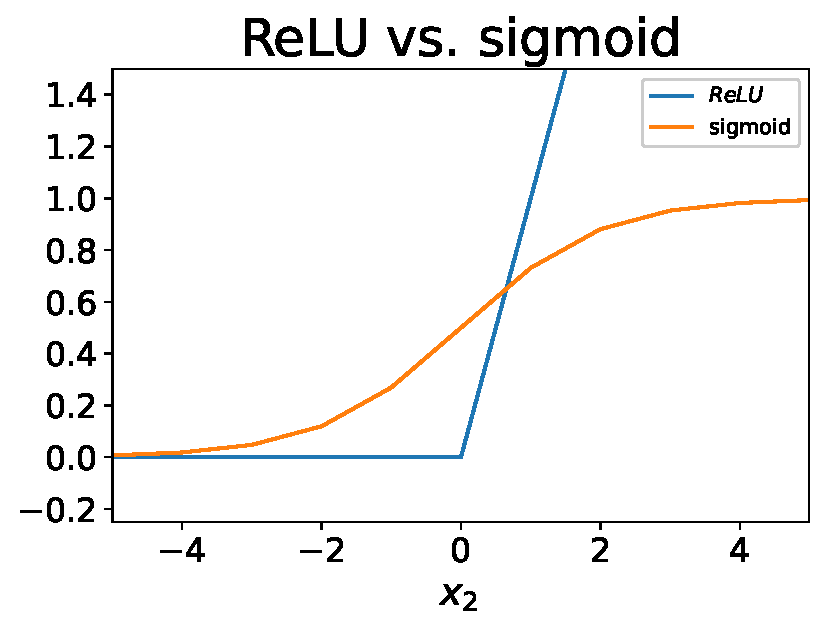
\includegraphics[width=.4\textwidth]{src/images/relu-vs-sigmoid.eps}
    \caption{Visualized comparison of $\ReLU$ (blue) and Sigmoid (orange). Sigmoid is evenly balanced between positive and negative values, whereas $\ReLU$ sets all values $f\left(\mybold{x^{(m)}}\right) < 0 \Rightarrow f\left(\mybold{x^{(m)}}\right) = 0$.}
    \label{fig:relu-vs-sigmoid}
\end{figure}
\\
\textbf{Softmax}\\
The previously mentioned \textit{Sigmoid} is used for binary classification with NNs.
The Softmax activation function allows for the classification task the usage of $N$ neurons in the output layer to compute probabilities of $N$ classes.
This is done by first computing the score $s_k(\mybold{x^{(m)}})$ of the input for each class $k$, then estimating the probability for each class by applying the Softmax function.
Let $f: \R^{N}\rightarrow [0, 1]^{K}$ with $B = [0, 1]$ be the Softmax, or unit, activation
\begin{align}
    f_k\left(\mybold{x^{(m)}}\right) = \frac{\e^{s_k(\mybold{x^{(m)}})}}{\sum \limits_{j=1}^K\e^{s_j(\mybold{x^{(m)}})}}
    \label{eq:softmax}
\end{align}
where $s$ represents the scoring function
\begin{align}
    s_k(\mybold{x^{(m)}}) = \skr{\mybold{\omega_k}, \mybold{x^{(m)}}} + \omega_{0,k}
\end{align}
with $\mybold{\omega_k}$ the $k$-th row-vector of $W$ and $\omega_{0,k}$ the $k$-th bias.
To then extract the class with the highest probability, the $\argmax$ method processes the output.
\subsubsection{Regularization}
To overcome the problem of overfitting the training data and improve convergence speed or overall generalization, Regularization methods can be applied to the NN.\\
\textbf{Kernel Regularization}\\
One idea is to apply Kernel Regularization.
Similar to the improvement of Ridge Regression over Linear Regression, the Kernel Regularization is essentially a mechanism to apply penalties to the weights of the Layer.
This causes the underlying model to have fewer degrees of freedom and therefore it gets harder for it to overfit the training data.
Using the $l_2$-regularization method for kernels in each training step the regularization term
\begin{align}
    L_r = \frac{\alpha}{2} \cdot \sum \limits_{j=1}^J \omega_j^2
\end{align}
gets calculated to then be added to the overall, and final, loss of the model for the iteration step.\\
\textbf{Dropout}\\
Another regularization method is Dropout.
Dropout is the method of randomly \textit{turning Neurons off}, which means, literally, to set the weight of several Neurons to $\omega_i = 0$, during training. This allows the model to be more robust during inference time and it proves to yield a more generalized solution~\cite{JMLR:v15:srivastava14a}.\\
\textbf{Batch Normalization (BN)}\\
BN was introduced in the a paper by Sergey Ioffe and Christian Szegedy~\cite{batch-normalization}.
It allows to configure much higher learning rates and be less careful about initialization.
It also acts as a regularizer, in some cases eliminating the need for Dropout.
Let $BN: \R^{B\times N} \rightarrow \R^{B \times N}$ be the BN transformation, with $B$ the batch size and $N$ the number of input features
\begin{align}
    \hat{x}_n^{(m)} = \frac{x_n^{(m)}-\mu^{(m)}}{\sqrt{\sigma_n^2 + \epsilon}}
    \label{eq:bn}
\end{align}
with
\begin{align}
    \mu^{(m)} = \frac{1}{B}\sum \limits_{n=1}^B x^{(m)}_n,
    \quad
    \sigma_n^2 = \frac{1}{B}\sum \limits_{n=1}^B\left(x^{(m)}_n-\mu^{(m)}\right)^2
\end{align}
where $\mu^{(m)}$ is the mean over the $B$ element batch and $\sigma_n^2$ the variance in the $n$-th feature.
\\
\textbf{Early Stopping}\\
A different way of regularization of the iterative learning algorithm is to stop the training process once the predictive power of the model reaches a minimum accepted value threshold.\\
\textbf{Learning Rate Schedule}\\
Another regularization method that is not directly applied to the training samples is called a learning rate schedule.
It adjusts the learning rate during the training process while following predefined rules.
Learning Rate Schedulers can be split into the groups of
\begin{multicols}{2}
\begin{enumerate}
    \item Power scheduling
    \item Exponential scheduling
    \item Piecewise constant scheduling
    \item\label{item:performance-scheduling} Performance scheduling
    \item 1cycle scheduling
\end{enumerate}
\end{multicols}
For this paper (\ref{item:performance-scheduling}) was selected.
It measures the validation error of the model every $s$ steps and reduces the learning rate $\eta$ by a factor of $\lambda$ when the error stops decreasing.
\subsection{Convolutional Neural Networks (CNNs)}\label{subsec:cnn}
Convolutional Neural Networks, short CNNs, are one type of architecture of feed forward NNs.
In contrast to ANNs, CNNs are capable of processing spatial data more suitably.
Due to this fact, CNNs are very popular for CV tasks.
They consist of layers, just like regular NN architectures, but with a twist.
Instead of connecting the input in each layer with neurons, CNNs connect the input neurons with \textit{feature maps} using \textit{receptive fields}, also called kernel filter masks.
Let $Y^{(l)}\in \R^{h^{(l)}\times w^{(l)}}$ be a receptive field were $h^{(l)}$ is the height and $w^{(l)}$ the width of the $l$-th kernel in a layer.
To generate the feature map for a conv. layer, $Y^{(l)}$ slides over regions of pixels, which is why it is called a sliding window, extracting features.
The step size used for sliding is called \textit{stride} and has a height and width parameter.
Additionally, a padding can be added to the input, which increases its size, but allows the kernel to process the borders as well.
The kernel size and the stride are both Hyperparameters.
Let a kernel in a conv. layer be described as $C^{(l)}: \R^{w^{(l)}_i \times h^{(l)}_i} \rightarrow \R^{w^{(l)}_o \times h^{(l)}_o}$ with $w^{(l)}_i$ and $h^{(l)}_i$ the width and height components of the input and $w^{(l)}_o, h^{(l)}_o$ and $d_o$ number of kernels, width height and depth components of the output, respectively.
\figref{fig:conv} visualizes this process, called a convolution~\footnote{A great explanation on how convolution works can be found in a video by the University of Nottingham (Computerphile) called \href{https://www.youtube.com/watch?v=C_zFhWdM4ic}{"How Blurs \& Filters Work - Computerphile"}, or the MIT lecture of Grant Sanderson \href{https://youtu.be/8rrHTtUzyZA}{"Convolutions in image processing"}.}.
\begin{figure}[!ht]
    \centering
    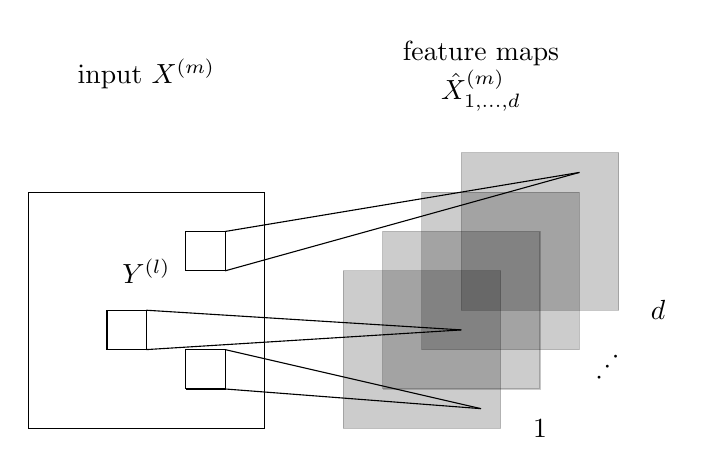
\begin{tikzpicture}
        \node at (1.5,4.5){input $X^{(m)}$};

		\draw (0,0) -- (3,0) -- (3,3) -- (0,3) -- (0,0);

		\draw (2,2) -- (2.5,2) -- (2.5,2.5) -- (2,2.5) -- (2,2);
		\draw (2,0.5) -- (2.5,0.5) -- (2.5,1) -- (2,1) -- (2,0.5);
		\draw (1,1) -- (1.5,1) -- (1.5,1.5) -- (1,1.5) -- (1,1);

		\draw (2.5,2) -- (7,3.25);
		\draw (2.5,2.5) -- (7,3.25);

		\draw (2.5,1) -- (5.75,0.25);
		\draw (2.5,0.5) -- (5.75,0.25);

		\draw (1.5,1.5) -- (5.5,1.25);
		\draw (1.5,1) -- (5.5,1.25);

		\node at (5.75,4.5){\begin{tabular}{c}{\begin{tabular}{c}feature maps\\ $\hat{X}_{1,\ldots,d}^{(m)}$\end{tabular}}\end{tabular}};

		\node at (1.5, 2) {$Y^{(l)}$};

		\node at (6.5, 0){$1$};
		\node at (7.25, 0.75){\rotatebox[origin=c]{90}{$\ddots$}};
		\node at (8, 1.5){$d$};


		\draw[fill=black,opacity=0.2,draw=black] (5.5,1.5) -- (7.5,1.5) -- (7.5,3.5) -- (5.5,3.5) -- (5.5,1.5);
		\draw[fill=black,opacity=0.2,draw=black] (5,1) -- (7,1) -- (7,3) -- (5,3) -- (5,1);
		\draw[fill=black,opacity=0.2,draw=black] (4.5,0.5) -- (6.5,0.5) -- (6.5,2.5) -- (4.5,2.5) -- (4.5,0.5);
		\draw[fill=black,opacity=0.2,draw=black] (4,0) -- (6,0) -- (6,2) -- (4,2) -- (4,0);
    \end{tikzpicture}
    \caption{Visualization of the functionality of a conv. layer. For each output feature map a kernel slides over the input to extract the features.}
    \label{fig:conv}
\end{figure}
To use CNNs to solve a specific task, such as classification or object detection, a fully connected multi layer Perceptron architecture processes the extracted features from the CNN to solve a specific task.
In this paper this MLP is called a task-solving-head.
The architectures implemented here and task-solving-heads are described further in "\nameref{subsec:model-architectures}".
A more detailed description and explanation of how the algorithm behind CNNs works can be found in~\cite{lecun-bengio}.
Also, the parameters to configure a CNN, e.g. the kernel size, the number of conv. layers, a regularization for the kernels or a dropout, are \nameref{subsubsec:hyperparameters}.\\
Let $C^{(l)}: \R^{H\times H}\times \R^{h\times w} \rightarrow \R^{(H-h)\times (H-w)}$ be the function of the $l$-th kernel in a layer that computes a convolution for a 2D input $X^{(m)}\in\R^{H\times H}$~\footnote{
    Note, this input has a single channel, like a feature map, or a single color channel in an RGB image.
}.
Then the full image $\hat{X}$ can be computed looping over each of the input elements $X_{i,j}$ by iterating with row index $i=1,\ldots, H-h$ and column index $j=1,\ldots, H-w$ and calculating
\begin{align}
    \hat{X}_{i,j}^{(m)} =
    \sum\limits_{s=1}^w
    \sum\limits_{r=1}^h
    X^{(m)}_{i+r, j+s}\cdot Y^{(l)}_{r,s}
\end{align}
here $X^{(m)}$ represents the $m$-th input matrix and $Y^{(l)}$ the $l$-th kernel of a layer.
This results e.g. in the first feature map of \figref{fig:conv}.\\
\textbf{Pooling}\\
Pooling can be used to reduce the shape, or the number of extracted feature maps of a CNN.
They can either reduce the height, with or depth components $h, w, d$, or reduce the number of extracted feature maps, which is called global pooling.\\
Let $Pool: \R^{k\times h_i\times w_i\times d_i}\rightarrow \R^{k\times h_o\times w_o\times d_o}$
be a function with $k$ the number of feature maps, $h_i, w_i, d_i$ the dimensions of each input feature map and $h_o, w_o, d_o$ the dimensions of the output feature maps respectively.\\
Global pooling combines neighboured feature maps and computes the average or max values accordingly.\newline
Let $Pool_G: \R^{n_i\times h\times w\times d} \rightarrow \R^{n_o\times h\times w\times d}$ be a global pooling function with $n_i$ the number of input feature maps, $n_o$ the number of output feature masks and $h,w,d$ as previously given.\\
To create a Deep CNN, different combinations of conv., pooling, BN layers, or layers with activation functions such as $\ReLU$ contain, can be stacked onto each.

\subsection{Losses}\label{subsec:losses}
Loss functions are a class of functions which map an input with one or many values to a real number.\\
Let $L$ be the loss function given as
$L(Y, {\hat{Y})}: \R^{M\times K}\times\R^{M\times K} \rightarrow \R$ with the predicted labels $\hat{Y}$ and the ground truth values $Y$.\\
During the training process, an optimization algorithm is used to adjust the model parameters in a way that minimizes the output of the loss function.
It does that by calculating the losses of current predictions in each step and uses their outputs to update the model parameters.
This makes the model eventually converge to a set of parameters, which map given input values $X$ onto the expected output $Y$ so that $\min L(Y,{\hat{Y}})$.
The following descriptions contain functions that calculate the loss of in a single prediction.

\subsubsection{Classification}\label{subsubsec:classification-loss}
\textbf{Logistic Loss (Cross-Entropy)}\\
For the classification task the most commonly applied function is the Logistic Loss, or Cross-Entropy~\cite{handsOn}.
The Cross-Entropy between two probability vector collections ${Y}$ the true label and $\hat{Y}$ the prediction, for $K$ classes, can be computed as
\begin{align}
    CE(Y, \hat{Y}) = - \sum \limits_{m=1}^M
    \skr{
        \mybold{y^{(m)}},     \log{\mybold{\hat{y}^{(m)}}}
    }
    \label{eq:cross-entropy}
\end{align}
This loss measures how distinguishable two probability are from each other.
The negative sum ensures that the loss decreases, when the distributions are closer to each other.\\
\textbf{Categorical Cross-Entropy}\\
Categorical CE, or softmax loss, is a combination of CE\eqref{eq:cross-entropy} and \eqref{eq:softmax}.
For Categorical CE it is required that the activation function of the layer prior to the output neurons is Softmax.
Here $\mybold{\hat{y}^{(m)}}$ and $\mybold{y}^{(m)}\in\{0,1\}^K$ are \textit{one-hot} encoded, as described with \eqref{eq:cropped-sample}.
Other than this requirement Categorical-CE~\eqref{eq:cross-entropy} is CE, the process is displayed in \figref{fig:cat-ce}.
\begin{figure}[!ht]
    \centering
    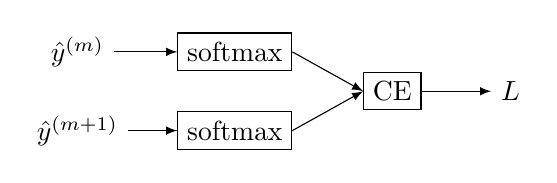
\begin{tikzpicture}
        \node(x) at (2.5, 1) {$\mybold{\hat{y}^{(m)}}$};
        \node(x2) at (2.5, 0) {$\mybold{\hat{y}^{(m+1)}}$};
        \node[draw, shape=rectangle](s) at (4.5, 1) {softmax};
        \node[draw, shape=rectangle](s2) at (4.5, 0) {softmax};
        \node[draw, shape=rectangle](c) at (6.5, 0.5) {CE};
        \node(y) at (8, 0.5) {$L$};

        \draw[->,-latex] (x) -- (s);
        \draw[->,-latex] (x2) -- (s2);
        \draw[->,-latex] (s.east) -- (c.west);
        \draw[->,-latex] (s2.east) -- (c.west);
        \draw[->,-latex] (c) -- (y);
    \end{tikzpicture}
    \caption{Visualization of Categorical-Cross-Entropy Loss. For each prediction softmax is computed, then the CE-loss over all predictions.}
    \label{fig:cat-ce}
\end{figure}
\subsubsection{Regression}\label{subsubsec:regression-loss}
The Loss functions to solve the regression task here can be split into a group of functions that compute distance based values, i.e. comparing vector values, and a group of functions that compares two dimensional objects, Bounding Boxes.
The former group consists of metrics using the commonly known $l_1$- and $l_2$-norm, the latter is based on  \textbf{I}ntersection \textbf{O}ver \textbf{U}nion, a geometric metric.\\
\textbf{Mean Average Error (MAE)}\\
MAE is a metric using the $l_1$-norm, it is computing its mean average, and given by
\begin{align}
    \MAE\left(Y, \hat{Y}\right) = \frac{1}{N}
    \sum \limits_{m=1}^M
    \norm{\mybold{y^{(m)}} - \mybold{\hat{y}^{(m)}}}_1\quad .
    \label{mae}
\end{align}
\textbf{Mean Square Error (MSE)}\\
As in "\nameref{subsec:linear-regression}" introduced MSE \eqref{eq:mse} is another metric for regression.\\\newline
Generally speaking the loss functions MAE and MSE are widely used regression-losses for tasks using tabular data, such as predicting house prices or detecting cancerous blood samples.
Because they compute distances between vectors MAE and MSE are not intuitively the best choice for BB regression.
The distance between vectors can be the same for two different vectors due to the definition of $l_1$ and $l_2$ norm.
To encode the location as well as the object within the predicted BB vector $\mybold{\hat{c}^{(m)}}$ a different loss function is required.
\\
\textbf{Intersection over Union (IoU)}\\
Intersection over Union, also called the Jaccard-Index, is one of the most popular evaluation metrics and losses applied in object detection. Other than previously introduced MAE, the IoU does not encode distances between vectors, but rather encodes the shape properties of the objects in comparison~\cite{GIoU}. Here it will encode the location, height and width of Bounding Boxes.
As its name suggests, IoU is computed from the area of intersection for each BBox prediction $\mybold{\hat{c}^{(m)}}$ with respect to its true Bounding Box values $\mybold{c^{(m)}}$ as well as the union of these.
Let
$
\mybold{c^{(m)}} = \begin{pmatrix}
        x^{(m)}_{\min},
        y^{(m)}_{\min},
        x^{(m)}_{\max},
        y^{(m)}_{\max}
\end{pmatrix}
$ be the ground truth coordinates of a Bounding Box
and
$\mybold{\hat{c}^{(m)}}=    \left(\hat{x}^{(m)}_{\min},\hat{y}^{(m)}_{\min},\hat{x}^{(m)}_{\max}, \hat{y}^{(m)}_{\max}\right)$
predicted coordinates by the regressor.
Then, the intersecting area, as seen in Figure~\ref{fig:iou}, can be computed from $w^{(m)}_I = \min(x^{(m)}_{\max}, \hat{x}^{(m)}_{\max}) - \max(x^{(m)}_{\min}, \hat{x}^{(m)}_{\min})$, the width of the intersection area, and $h^{(m)}_I = \min(y^{(m)}_{\max}, \hat{y}^{(m)}_{\max})-\max(y^{(m)}_{\min}, \hat{y}^{(m)}_{\min})$, the respective height.

\begin{figure}[!ht]
    \centering
\begin{minipage}{0.28\textwidth}
    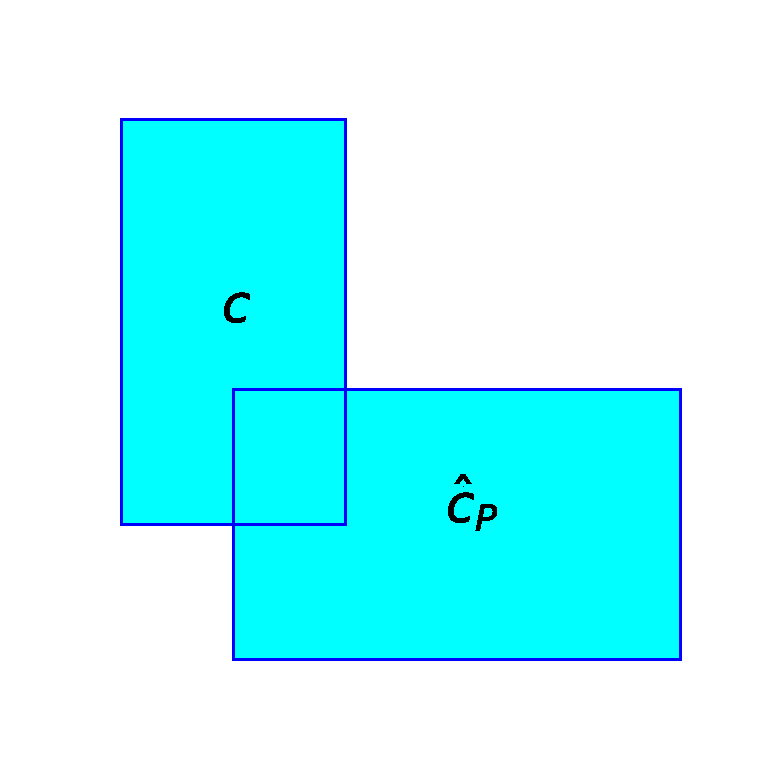
\includegraphics[width=\textwidth]{src/images/iou-plot-union.eps}
\end{minipage}
\begin{minipage}{0.28\textwidth}
    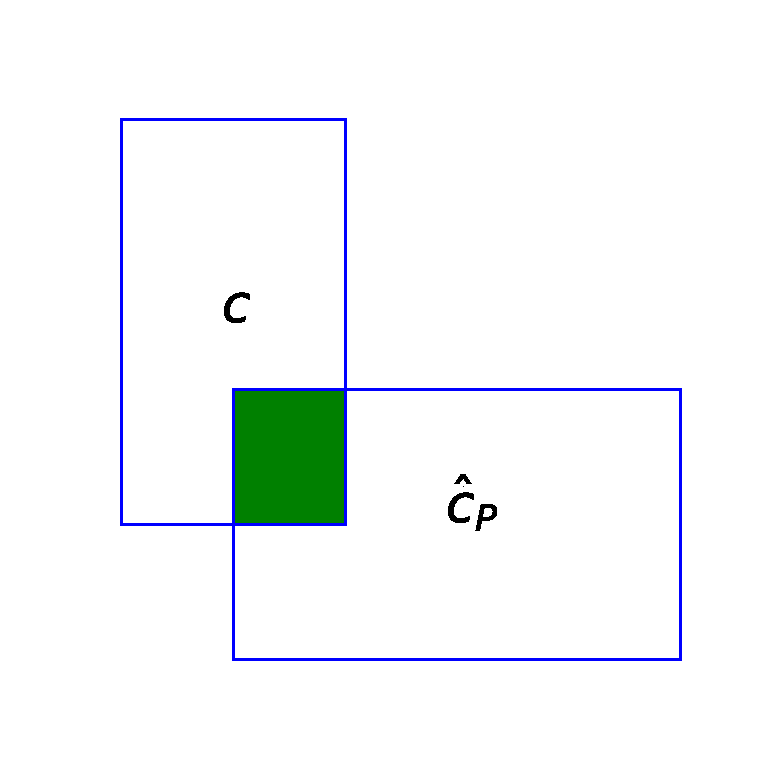
\includegraphics[width=\textwidth]{src/images/iou-plot-intersection.eps}
\end{minipage}
\begin{minipage}{0.28\textwidth}
    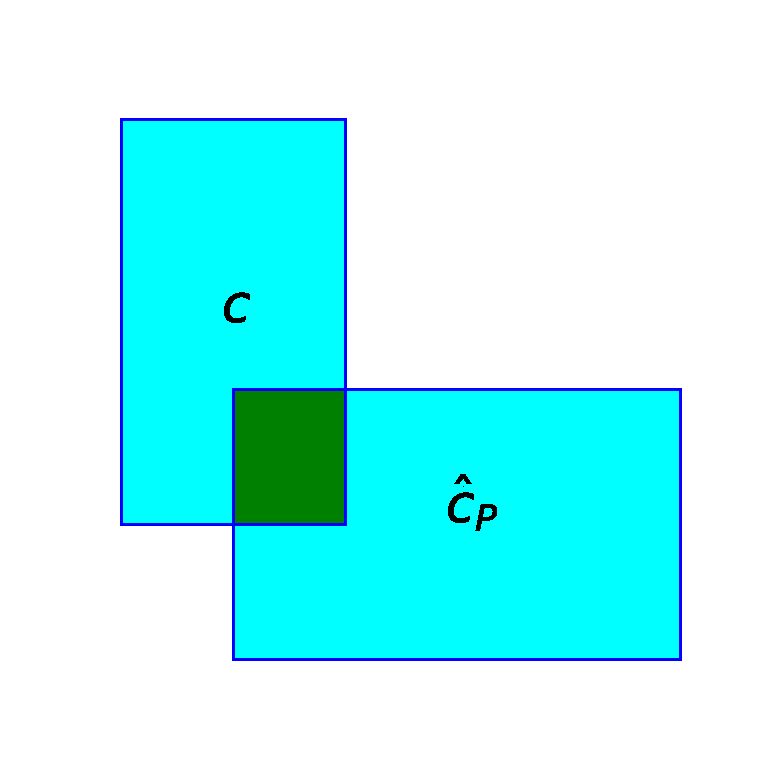
\includegraphics[width=\textwidth]{src/images/iou-plot-all.eps}
    \end{minipage}
    \caption{Left: $A^{(m)}_I$ (green) in combination with $A^{(m)}_U$ (cyan and green). Center: The intersection area $A^{(m)}_I$. Right: The union area $A^{(m)}_U$ for two BBs.}
    \label{fig:iou}
\end{figure}
%\end{paracol}
\begin{align}
    A^{(m)}_I &= h^{(m)}_I \cdot w^{(m)}_I
\end{align}
Using $A^{(m)}_I$, the area of union, $A^{(m)}_U$ can be computed, visualized in Figure~\ref{fig:iou} (center).
Let $h^{(m)}_c = x^{(m)}_{\max}-x^{(m)}_{\min}$ be the height of the ground truth, $w^{(m)}_c = y^{(m)}_{\max}-y^{(m)}_{\min}$ the corresponding width and $h^{(m)}_{\hat{c}}=\hat{x}^{(m)}_{\max}-\hat{x}^{(m)}_{\min}$ the height of the predicted Bounding Box with $w^{(m)}_{\hat{c}} = \hat{y}^{(m)}_{\max}-\hat{y}^{(m)}_{\min}$.
Then, the union area can be computed by subtracting the intersection area $A^{(m)}_I$ from the sum of the areas within the BBs
\begin{align}
    A^{(m)}_U = (h^{(m)}_c\cdot w^{(m)}_c) + (h^{(m)}_{\hat{c}} \cdot w^{(m)}_{\hat{c}}) - A^{(m)}_I\quad .
\end{align}

To compute the IoU, $A^{(m)}_I$ is devided by $A^{(m)}_U$
\begin{align}
    \IoU(\mybold{c}^{(m)}, \mybold{\hat{c}^{(m)}}) = \frac{A^{(m)}_I}{A^{(m)}_U}\quad .
    \label{eq:iou}
\end{align}
This concept can be easier described using images.
As visualized in \figref{fig:iou}, the function computes the ratio of intersecting area over the union area.\newline
The IoU can be used as a loss function by simply calculating $L^{(m)}_{\IoU}\left(\mybold{c^{(m)}}, \mybold{\hat{c}^{(m)}}\right) = 1 - \IoU\left(\mybold{c^{(m)}}, \mybold{\hat{c}^{(m)}}\right)$.
This is also called the Jaccard distance, measures the dissimilarity in the objects and can be a target of minimization, whereas IoU is $1$ when $\mybold{\hat{c}^{(m)}}=\mybold{c}^{(m)}$ .\\
To calculate the $\IoU_B$, the IoU over a batch of predictions, the average is computed
\begin{align}
    \IoU_B\left(
        \mybold{c^{(m)},
        \mybold{\hat{c}^{(m)}}
    }\right) = \frac{1}{M}
    \sum\limits_{m=1}^M
    \IoU\left(
        \mybold{c^{(m)},
        \mybold{\hat{c}^{(m)}}
    }\right)
\end{align}
\textbf{Generalized Intersection over Union (GIoU)}\\
\begin{wrapfigure}{r}{0.5\textwidth}
    \centering
    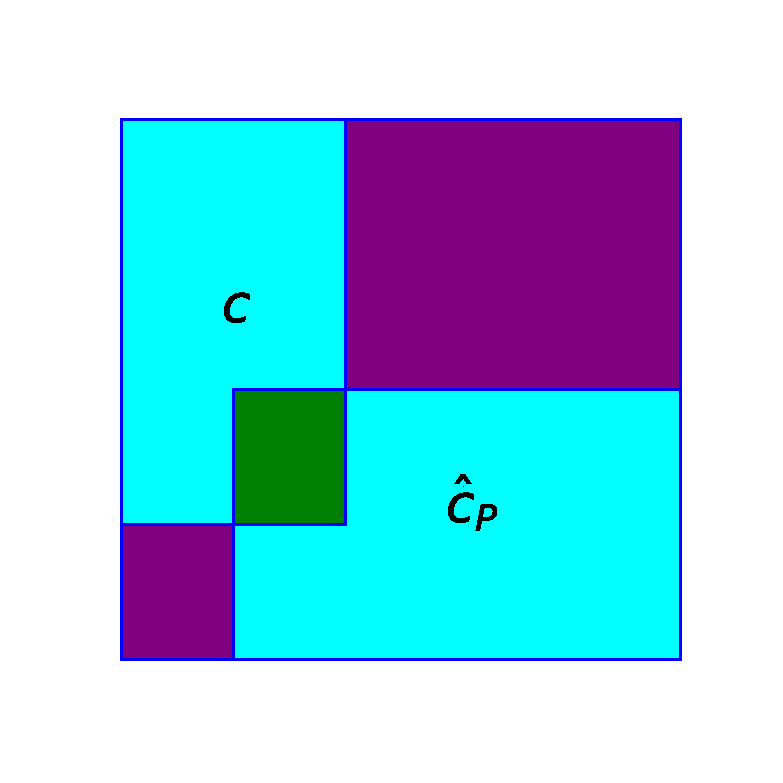
\includegraphics[width=.25\textwidth]{src/images/giou-plot.eps}
    \caption{$A_I$ (green), $A_U$ (cyan and green) and $A_C$ (purple + cyan + green)}
    \label{fig:giou}
\end{wrapfigure}
In the 2019 paper by Rezatofighi et al.~\cite{GIoU} the researchers found out that using a modified version of the regular \textit{IoU} for axis aligned 2D bounding boxes – so called \textit{Generalized Intersection over Union (GIoU)} – improves predictions drastically.\\
The GIoU is calculated by subtracting the share of non overlapping area
\begin{align}
    \frac{A^{(m)}_C - A^{(m)}_U}{A^{(m)}_C}
\end{align}
with $A^{(m)}_C$ the area of the smallest convex hull or shape around the two Bounding Boxes. Let $\mybold{\bar{c}^{(m)}} = \left(\bar{x}^{(m)}_{\min}, \bar{y}^{(m)}_{\min}, \bar{x}^{(m)}_{\max}, \bar{y}^{(m)}_{\max}\right)$ be to coordinates of the convex hull
with
\begin{align*}
    \bar{x}^{(m)}_{\min} &= \min(x^{(m)}_{\min}, \hat{x}^{(m)}_{\min})\\
    \bar{y}^{(m)}_{\min} &= \min(y^{(m)}_{\min}, \hat{y}^{(m)}_{\min})\\
    \bar{x}^{(m)}_{\max} &= \max(x^{(m)}_{\max}, \hat{x}^{(m)}_{\max})\\
    \bar{y}^{(m)}_{\max} &= \max(y^{(m)}_{\max}, \hat{y}^{(m)}_{\max})
\end{align*}
and $A^{(m)}_C = (\bar{x}^{(m)}_{\max} - \bar{x}^{(m)}_{\min}) \cdot (\bar{y}^{(m)}_{\max} - \bar{y}^{(m)}_{\min})$. In combination with the IoU
\begin{align}
    \GIoU\left(
        \mybold{c^{(m)}},
        \mybold{\hat{c}^{(m)}}
    \right) =
    \IoU\left(
        \mybold{c^{(m)}},
        \mybold{\hat{c}^{(m)}}
    \right)
    - \frac{A^{(m)}_C - A^{(m)}_U}{A^{(m)}_C}\quad.
    \label{eq:giou}
\end{align}
A visualization of these areas can be seen in Figure~\ref{fig:giou}.
The corresponding loss function is
\begin{align}
    L_{\GIoU}
    \left(
        \mybold{c^{(m)}},
        \mybold{\hat{c}^{(m)}}
    \right) = 1 - \GIoU\left(
        \mybold{c^{(m)}},
        \mybold{\hat{c}^{(m)}}
    \right)\quad .
\end{align}
In the same way, like the IoU, is GIoU a similarity measure.
Additionally, it is capable calculate this measure for objects without overlap.
\subsection{Performance metrics}\label{subsec:metrics}
As in previous sections briefly described metrics are a group of functions, similar to Losses, that estimate the current predictive power of a ML Method.
Like in the case of the loss, it is desired that the fitted function optimizes these metrics.
Some metrics, like the \textit{Accuracy} of right predictions or \textit{GIoU} need to be maximized, some metrics, such as the \textit{RMSE} get minimized, but all metrics measure or monitor the performance of the model during and after training.
The following section will introduce metric functions implemented here, and will address some of their trade-offs.

\subsubsection{Classification}
\textbf{Confusion Matrix}\\
For the classification task a widely used metric is the Confusion Matrix.
The Confusion Matrix contains rows for actual classes and columns for predicted classes for each of the available output classes.
The cells contain the number of occurrences of each pair of row and column value.\\
As an example, consider the results of binary classification for the classes "Cole\-optera" and "not Cole\-optera".
If the model predicts "Cole\-optera" for images containing "Cole\-optera" the result is called a True Positive (TP) prediction, a predicted label of "not Cole\-optera" for the same image is called a False Positive (FP).
For images of class "not Cole\-optera", on the other hand, predictions of "not Cole\-optera" are called True Negatives (TN) and "Coleoptera" False Negatives (FN). Then, the resulting parameterised confusion matrix would look as following.
\begin{center}
    \begin{tabular}{|c|c|c|}
        \hline
        & Coleoptera & not Coleoptera \\
        \hline
        Coleoptera     & TP          & FN              \\
        \hline
        not Coleoptera & FP          & TN              \\
        \hline
    \end{tabular}
\end{center}
Albeit this example is using binary classification, the confusion matrix is not limited to two classes and can be computed for multi-label classification, as well.\\
The values in the resulting confusion matrix can be leveraged to calculate other metrics, such as the total number of correct predictions, or the total number of false predictions.
These values, in turn, can be applied to calculate other metrics such as Precision, Recall and the Accuracy.\\
\textbf{Precision and Recall}\\
To measure the Precision of a classifier the formula is given by
\begin{align}
    precision = \frac{TP}{TP+FP}\quad.
    \label{eq:precision}
\end{align}
According to this formula, the Precision computes how many predicted positive labels are indeed positive, but it ignores False Negative predictions.
In some cases it is important to consider these False Positive predictions, to do so the Precision is used in combination with the Recall.
The Recall is given by
\begin{align}
    recall = \frac{TP}{TP+FN}
    \label{eq:recall}
\end{align}
Also called the sensitivity or \textit{True Positive rate}, it is the ratio of positive instances that are correctly detected by the classifier.
Recall is a measure of how many of the truly positive labels were labeled positive by the classifier.\\
\textbf{$F_1$}\\
Sometimes it is desired to combine Precision and Recall in one metric, this is called the $F_1$ \textit{score}. The $F_1$ score is the harmonic mean of precision and recall
\begin{align}
    F_1 = \frac{2}{\frac{1}{precision} + \frac{1}{recall}} = 2 \cdot \frac{precision \cdot recall}{precision + recall} = \frac{TP}{TP + \frac{FN+FP}{2}}
    \label{eq:f1}
\end{align}
Unfortunately, due to the fact that this metric is a combination of precision and recall it is impossible to optimize it to maximize both values, this is called the \textit{precision-recall tradeoff}.\\
\textbf{Accuracy}\\
The Accuracy can be computed by dividing the number of correct predictions by the total number of predictions
\begin{align}
    ACC = \frac{
        \text{TP} + \text{TN}
    }{
        \text{TP} + \text{TN} + \text{FP} + \text{FN}
    }
    \label{eq:accuracy}
\end{align}


\subsubsection{Regression}\label{subsubsec:regression-metrics}
The standard metric applied for regression tasks is the $\MSE$ \eqref{eq:mse}~\cite{handsOn}, or its easier to interpret the \textit{R}oot Mean Squared Error ($\RMSE$).\\
\textbf{Root Mean Squared Error (RMSE)}\\
RMSE has the form
\begin{align}
    \RMSE\left(Y, \hat{Y}\right) =
    \sqrt{\frac{1}{M}\sum \limits_{m=1}^{M}\norm{\mybold{y^{(m)}} - \mybold{\hat{y}^{(m)}}}_2^2}
    \label{eq:rmse}
\end{align}
and is considered to be easier to interpret for humans than the MSE due to its scale in codomain.\\
\textbf{(G)IoU}\\
As in "\hyperref[subsubsec:regression-loss]{Regression Losses}" mentioned, \textit{IoU}-Loss and \textit{GIoU}-Loss originated from the metrics \textit{IoU} and \textit{GIoU}.
They can be easily calculated back to the original form
\begin{align}
    \GIoU(Y, \hat{Y}) &= 1 - L_{\GIoU}(Y, \hat{Y})\\
    \IoU(Y, \hat{Y}) &= 1 - L_{\IoU}(Y, \hat{Y})
\end{align}
For the regression tasks in this paper, the GIoU in combination with the RMSE is computed, to ensure own implementations of wrappers for the GIoU calculation are correct.
\subsection{Training Strategies}\label{subsec:training-strategies}
Amongst the supervised training algorithms, we can differentiate the training strategies for the problem of localization and classification of insects into two groups. Whereas one group of strategies trains two separate models ("\nameref{subsubsec:2-model-strategy}") to solve the detection task, the other uses a 1-stage approach ("\nameref{subsubsec:2-in-1-model-strategy}") where one model is used to solve the task.
In supervised learning and for all of the following strategies the objective is equal: a loss function gets optimized until it reaches a satisfying threshold from which on the predictions are considered accurate enough or within the required boundaries, as described before in the previous section "\nameref{subsec:losses}".

\subsubsection{2-Stage-Model-Strategies}\label{subsubsec:2-model-strategy}
The former group, further called 2-Stage-Model-Strategies, includes independent training and sequential training training. All 2-Stage-Strategies search for solutions of two different optimization problems.\\
Let  $g: \R^{N} \rightarrow \R^{4}$ be the bounding box predictor, $f: \R^{N} \rightarrow \R$ be the classifier and $h$ the cropping and resizing function \eqref{eq:crop}.\\
Therefore, we calculate at inference for the $m$-th input
\begin{align}
    \mybold{\hat{y}^{(m)}} =
    \hat{f}\left(
        h\left(
            \mybold{x^{(m)}},
            \hat{g}\left(
                \mybold{x^{(m)}}
            \right)
        \right)
    \right)
\end{align}
\textbf{Independent Training}:
When training $f$ and $g$ independently, we solve the optimization problems for each model separately.
The optimization task for the BB regressor is
\begin{align}
    \hat{g} =
    \argmin_g
    \frac{1}{M}
    \sum \limits_{m=1}^M
        L_{\text{bbox}}\left(
            g\left(
                \mybold{x^{(m)}},
                \mybold{c^{(m)}}
            \right)
        \right)
    \label{eq:independent-g-loss}
\end{align}
with $L_{\text{bbox}} = 1 - \GIoU$ the $L_{GIoU}$, as described in "\nameref{subsubsec:regression-metrics}".
Both models get trained on individual data sets, the Regressor on \eqref{eq:regression-sample} and the Classifier on \eqref{eq:classification-sample} respectively.

And the minimization of the classification-loss
\begin{align}
    \hat{f} =
    \argmin_{f}
    \frac{1}{M}
    \sum \limits_{m=1}^M
    L_y\left(
        f\left(
            h\left(
                \mybold{x^{(m)}},
                \mybold{c^{(m)}}
            \right)
        \right),
        \mybold{y^{(m)}}
    \right) \quad .
\end{align}
The two models get trained independently, each on a data sets containing labels of the related shapes \eqref{eq:classification-sample} and \eqref{eq:regression-sample}, to be later combined into a independent two-stage-model.\\
\textbf{Sequential Training}:
For Sequential Model training, the same optimization for the regression-loss $\hat{g}$ is used as previously described in the independent training approach \eqref{eq:independent-g-loss}.
For the classification task, the loss
\begin{align}
    \hat{f} =
    \argmin_{f}
    \frac{1}{M}
    \sum \limits_{m=1}^M L_y\left(
        f\left(
            h\left(
                \mybold{x^{(m)}},
                \hat{g}\left(
                    \mybold{x^{(m)}}
                \right)
            \right),
            \mybold{y^{(m)}}
        \right)
    \right)
\end{align}
gets optimized.
Where $\hat{g}\left(\mybold{x^{(m)}}\right)$ is the predicted BBox coordinates from the already fitted regressor.
This strategy requires finding a fitting solver for the regression task first, then training the classification method upon a training set generated by the regressor.
\subsubsection{Single-Stage-Model-Strategy}\label{subsubsec:2-in-1-model-strategy}
To solve the classification and localization task in a single pass through the network, a different approach is chosen.
Let $f: \R^{N}\rightarrow \R^4\times \R$ be the object detector (visualized in \figref{fig:parallel-heads}).
Then the loss calculated for the network is given by
\begin{align}
    \hat{f} =
    \argmin_f
    \frac{1}{M}
    \sum \limits_{m=1}^M
    \left[
        L_y\left(f_2(\mybold{x^{(m)}}), \mybold{y^{(m)}}\right)
        +
        \lambda
        L_{\text{bbox}}\left(
            f_1\left(\mybold{x^{(m)}}\right),
            \mybold{c^{(m)}}
        \right)
    \right]
\end{align}
\begin{figure}[!ht]
    \centering

    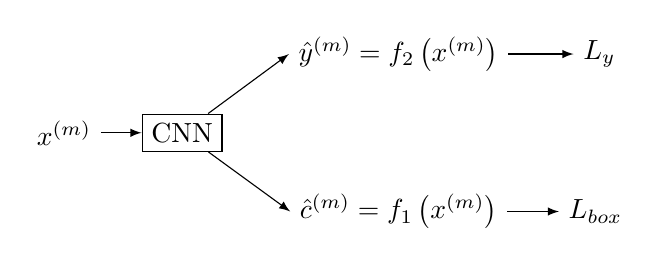
\begin{tikzpicture}

        % Set A
        \node (x) at (0,1){$\mybold{x^{(m)}}$};

        % Set B
        \node[draw, rectangle] (CNN) at (1.5,1){CNN};

        \node (c) at (4.25,0){$\mybold{\hat{c}^{(m)}} = f_1\left(\mybold{x^{(m)}}\right)$};
        \node (L_b) at (6.75, 0) {$L_{\text{box}}$};

        \node (y) at (4.25,2) {$\mybold{\hat{y}^{(m)}} = f_2\left(\mybold{x^{(m)}}\right)$};
        \node (L_y) at (6.8, 2) {$L_{y}$};

        \draw[-latex] (x) -- (CNN);
        \draw[-latex] (CNN) -- (c.west);
        \draw[-latex] (c) -- (L_b);
        \draw[-latex] (CNN) -- (y.west);
        \draw[-latex] (y) -- (L_y);
    \end{tikzpicture}
    \caption{single-stage-model: The input gets processed by a single CNN, the resulting features are used by a Classification- and Regression-Head.}
    \label{fig:parallel-heads}
\end{figure}
Where $f$ is again the classifier, $g$ the bounding box regressor and $\mybold{y^{(m)}}$ and $\mybold{c^{(m)}}$ the ground truth labels yielded from a data set with samples in the shape \eqref{eq:1-stage-sample}.
This architecture does not crop the image during inference time, which can be a potential speed improvement.
Using the parameter $\lambda$ the losses can be weighted differently.
Sometimes the losses of the outputs differ in their codomain.
This can be solved using the weight parameter $\lambda$ to scale $L_{\text{bbox}}$ accordingly.
The here used configuration is based on equal weighted losses, $\GIoU$ and \eqref{fig:cat-ce} share almost the same codomain, so no further weights were introduced and $\lambda = 1$ fixed set.

\subsection{Model Optimization}\label{subsec:model-optimization}
\subsubsection{Hyper Parameters}\label{subsubsec:hyperparameters}
Hyper Parameters (HPs) are parameters used to configure the model prior to the training phase.
Commonly used HPs are the learning rate of the optimization algorithm, regularization parameters for underlying layers of the model or the batch size used to feed the training data into the model.


\subsubsection{Hyper Parameter Optimization}\label{subsubsec:hpo}
For the task of Hyper Parameter Optimization (HPO), several optimization techniques and algorithms are available.
Amongst broad random parameter initialization, so called Random Search, more sophisticated algorithms were build to find the best parameter combination for the model to solve its task with the minimal loss.
Let $L(y,\hat{y})$ be the loss function measuring the model's predictive power, then it is desired to find $\mybold{\hat{\theta}}$ the vector of hyper parameters with minimal loss
\begin{align}
    \mybold{\hat{\theta}} = \argmin_{\mybold{\theta}} L_{\mybold{\theta}}(Y, \hat{Y})
\end{align}
with $\mybold{\theta}$ the vector of hyper parameters.\\
Grid search is the most naive HPO method, in which a grid of HP combinations gets created and evaluated on each step.
Unfortunately, this method naively evaluates  all points in this equidistant grid, without any restrictions.
In order to speed up the HPO process and use a more sophisticated method evaluating these HPs Bayesian Optimization~\cite{BayesianOptimization} was used.\\
For this the implementation of \path{keras-tuner}'s~\cite{omalley2019kerastuner} \path{BayesianOptimization} was integrated.\\
\path{BayesianOptimization} allows configuration of an objective \path{objective} that the optimizer optimizes, \path{num_initial_points} the number of starting points in the Bayes parameter space, \path{max_trials} the number of maximum total trials and \path{seed} a seed value to replicate the experiments.
For this paper the validation accuracy was optimized for classifiers and the validation loss ($L_{\GIoU}$) for regressors.
Each of the HPO iterations used $12$ initial points and performed a total of $36$ trials.
For all experiments the seed of $42$ was applied.

The optimized HPs per task can be found in \figref{fig:reg-hp-table} and \figref{fig:clf-hp-table}.
Another method to optimize the HPs is cross-validation. This method was not applied in this paper, due to the fact that it was not possible to implement it for the case of \nameref{subsubsec:2-model-strategy}, because the classifier receives the pretrained weights of the regressor.
